\documentclass[11pt]{article}
\usepackage[margin=1in]{geometry}
\usepackage{graphicx}
\usepackage{booktabs}
\usepackage{amsmath,amssymb}
\usepackage{microtype}
\usepackage{hyperref}
\usepackage{xcolor}
\usepackage{enumitem}
\usepackage[T1]{fontenc}
\usepackage[utf8]{inputenc}
\usepackage{float}
\usepackage{longtable}
\usepackage{caption}
\usepackage{tikz}
\usepackage{setspace}
\onehalfspacing

\graphicspath{{../results/figures/}}

\title{\textbf{Detailed Project Report}\\[6pt]
\Large Dispersion, Not Displacement:\\
Loss of Alveolar Epithelial State Coherence in Lethal COVID-19}
\author{Pierce Taylor \& Chimdi Walter Ndubuisi\\
Computational Systems Biology 8190\\
Dr.\ Toni Kazic}
\date{\today}

\begin{document}
\maketitle

\tableofcontents
\clearpage


% ============================================================================
\section{Executive Summary}
% ============================================================================

This report documents a computational systems biology project investigating how alveolar epithelial cells fail in lethal COVID-19. Using single-nucleus RNA sequencing data from 22,128 alveolar cells across 27 donors (Melms et al., 2021), we tested two competing geometric models of epithelial injury: (1) coherent displacement, in which all injured cells shift toward a single damaged state, and (2) heterogeneous dispersion, in which cells scatter across multiple injury states simultaneously.

Our principal finding is that lethal COVID-19 produces \textbf{dispersion-dominated loss of alveolar epithelial state coherence}. COVID-19 cells occupy a 2.3-fold broader region of gene-expression space than healthy cells (Levene $p < 10^{-30}$), while centroid displacement is absent ($p = 1.0$). This dispersion finding replicates decisively in an independent cohort of 89,736 cells from 618 donors across 35 datasets (variance ratio 1.65; $p \approx 10^{-137}$). The project's contribution is primarily methodological: pre-registered opposing hypotheses, ten systematic ablations, donor-level modeling, portable continuous state scores, and honest reporting of which findings survive and which do not.


% ============================================================================
\section{Introduction and Scientific Question}
% ============================================================================

\subsection{Biological Context}

The lungs contain approximately 480 million microscopic air sacs called alveoli. Each alveolus is lined by a thin sheet of epithelial cells---the alveolar epithelium---where oxygen crosses into the blood. Two cell types compose this sheet:

\begin{description}[style=nextline]
\item[AT1 cells (Alveolar Type 1)] Very thin, very flat cells covering approximately 95\% of the alveolar surface. They form the gas-exchange barrier. AT1 cells do not divide.
\item[AT2 cells (Alveolar Type 2)] Smaller, cube-shaped cells that perform two critical functions: (i) secreting pulmonary surfactant, a soapy substance that prevents alveoli from collapsing during exhalation; and (ii) serving as local stem cells that divide and differentiate into new AT1 cells when the existing AT1 population is damaged.
\end{description}

The AT2-to-AT1 differentiation process passes through a transient intermediate state characterized by expression of KRT8, CLDN4, and SFN. These transitional cells---also called damage-associated transient progenitors (DATPs)---are rare in healthy lungs but accumulate during injury when cells become stuck mid-transition.

\subsection{Why COVID-19 is Catastrophic for This System}

SARS-CoV-2 enters AT2 cells through the ACE2 receptor. This is doubly catastrophic because it compromises both the surfactant-producing cells (leading to alveolar collapse) and the regenerative progenitor pool (preventing AT1 replacement). The body's inflammatory response inflicts additional collateral damage. In lethal cases, autopsies reveal diffuse alveolar damage: holes in the AT1 sheet, edema, and abnormal cells caught mid-transition.

\subsection{The Specific Question}

Previous studies (Melms et al., 2021; Delorey et al., 2021) already described alveolar injury in COVID-19 lungs using cluster-based approaches. Our project asks a more specific geometric question:

\begin{quote}
\textbf{When the alveolar epithelium fails in lethal COVID-19, does it fail in a coordinated way (every sick cell moves toward one damaged state), or in a dispersed way (cells scatter in many different directions at once)?}
\end{quote}

These two possibilities---coherent displacement versus heterogeneous dispersion---make opposite geometric predictions:

\begin{itemize}
\item \textbf{Coherent displacement}: The group center (centroid) of COVID-19 cells shifts away from healthy cells. Within-group variance remains unchanged.
\item \textbf{Heterogeneous dispersion}: The centroid may not move much, but the spread of COVID-19 cells increases dramatically. Cells scatter in many directions without converging on a single damaged state.
\end{itemize}

By pre-specifying both tests, we ensure that whichever test fails is as informative as whichever succeeds. A failing test rules out a specific mechanism.

\subsection{Nature of the Contribution}

This project is not a biology-discovery paper. We are not claiming to discover new effects of COVID-19 on lung tissue. The contribution is \textbf{methodological}:

\begin{enumerate}
\item Pre-registered geometric tests with mutually exclusive predictions
\item Ten systematic ablation analyses to separate robust from fragile findings
\item Independent 618-donor cross-cohort replication
\item Donor-level modeling that properly treats 27 donors (not 22,128 cells) as the sample size
\item Portable continuous state scores that transfer across cohorts
\item Mechanistic decomposition identifying which gene programs drive the dispersion
\item Honest reporting of which findings survive and which do not
\end{enumerate}


% ============================================================================
\section{Data Sources}
% ============================================================================

\subsection{Primary Cohort: Columbia/NYP COVID-19 Lung Atlas (SCP1219)}

The primary dataset is a publicly released single-nucleus RNA-seq atlas of post-mortem lung tissue from patients who died of COVID-19, plus healthy organ donors as controls (Melms et al., 2021).

\begin{center}
\small
\begin{tabular}{ll}
\toprule
Attribute & Value \\
\midrule
Total nuclei sequenced & 116,313 \\
Assay & 10x Genomics 3' v3 snRNA-seq \\
Total donors & 27 (7 healthy + 20 COVID-19) \\
Alveolar epithelial cells after subsetting & 22,128 \\
\quad AT1 cells & 9,608 \\
\quad AT2 cells & 11,341 \\
\quad ECM-high transitional cells & 1,179 \\
Per-donor cell counts & Range 62--2,850 \\
Donors with $<$300 cells & 10 of 27 \\
\bottomrule
\end{tabular}
\end{center}

\textbf{Critical statistical note}: The true sample size is \textbf{27 donors}, not 22,128 cells. Cells from the same donor share the same biology and are not independent observations. Every statistical claim in this project must hold at the donor level.

\subsection{Independent Replication Cohort: cellxgene Census}

For independent replication, we constructed a second dataset from the CZ cellxgene census---a curated federation of single-cell datasets:

\begin{center}
\small
\begin{tabular}{ll}
\toprule
Attribute & Value \\
\midrule
Total alveolar AT1/AT2 cells & 89,736 (after per-donor subsampling) \\
Total donors & 618 (43 COVID-19 + 575 normal) \\
Number of independent datasets & 35 \\
Per-donor cap & 200 cells \\
Gene panel & 84 genes (programs + canonical markers) \\
SCP1219 exclusion & Excluded by dataset ID \\
\bottomrule
\end{tabular}
\end{center}

The primary cohort was excluded by its dataset identifier, ensuring zero data leakage between primary and replication analyses. The 84-gene panel is sufficient to score gene programs and compute dispersion but too narrow to build an independent manifold or run trajectory analysis from scratch.


% ============================================================================
\section{Computational Pipeline}
% ============================================================================

The entire analysis is implemented in Python 3.12.3 using Scanpy 1.12.1, with all parameters stored in a single \texttt{config.yaml} file and a fixed random seed of 42 for full reproducibility.

\subsection{Step 1: Quality Control}

Nuclei were filtered using standard thresholds to remove artifacts:
\begin{itemize}
\item $\geq$200 genes per cell (removes empty droplets)
\item $\leq$8,000 genes per cell (removes doublets---two cells captured together)
\item $\leq$20\% mitochondrial reads (removes dying/damaged cells)
\item Genes detected in $<$10 cells were dropped
\end{itemize}

\subsection{Step 2: Subset to Alveolar Epithelium}

Using the atlas's pre-computed cell-type labels, we retained AT1, AT2, and ECM-high epithelial (transitional) cells. Labels were validated by confirming that canonical marker genes (SFTPC in AT2, AGER in AT1, KRT8/CLDN4 in transitional) were expressed at expected levels in the correct populations.

\subsection{Step 3: Normalization and Log-Transformation}

\begin{enumerate}
\item \textbf{Library-size normalization}: Each cell's expression vector was rescaled to sum to 10,000 counts, removing sequencing depth differences.
\item \textbf{Log-transformation}: $\log(1+x)$ was applied to compress dynamic range and approximate normality.
\item \textbf{Raw preservation}: The full log-normalized matrix was stored in \texttt{adata.raw} for gene-program scoring.
\end{enumerate}

\subsection{Step 4: Highly Variable Gene Selection}

The 3,000 most biologically variable genes were selected using the Seurat v3 method. The remaining $\sim$17,000 genes contribute mostly noise and are excluded from downstream dimensionality reduction.

\subsection{Step 5: Scaling and PCA}

Each gene was scaled to mean 0 and variance 1 (clipped at 10 to prevent outlier domination). Principal Component Analysis (PCA) reduced each cell from $\sim$3,000 HVG dimensions to 50 principal components. After this step, every cell is represented as a 50-number vector.

\subsection{Step 6: Batch Correction with Harmony}

Harmony was applied using \texttt{donor\_id} as the batch key to remove systematic technical differences between donors while preserving genuine biological variation. The algorithm converged in 3 iterations, producing corrected coordinates in \texttt{X\_pca\_harmony}.

\textbf{The Harmony Bug}: An important debugging episode occurred during development. The Harmony Python library changed its output format between CPU and PyTorch backends: the old CPU backend returned a matrix shaped (PCs $\times$ cells), while the new PyTorch backend returns (cells $\times$ PCs). Our wrapper always transposed, which was correct for the old backend and wrong for the new one. The fix was a one-line shape check. Post-fix, the pseudotime shift amplified from $+0.048$ to $+0.125$ (2.6$\times$). This episode demonstrates that ``batch correction didn't help'' can mean ``the implementation is broken,'' and it was caught through systematic ablation testing.

\subsection{Step 7: Graph Construction and Embeddings}

\begin{enumerate}
\item \textbf{$k$-nearest neighbor graph}: Each cell was connected to its 15 nearest neighbors in PCA space, forming the graph on which all downstream analyses operate.
\item \textbf{UMAP}: A 2D layout for visualization only. UMAP distorts distances and is never used for statistical testing.
\item \textbf{Diffusion map}: A 15-component coordinate system based on random-walk distances on the cell graph, designed for trajectory analysis.
\end{enumerate}

\subsection{Step 8: Diffusion Pseudotime (DPT)}

A root cell was selected as the cell closest to the centroid of all healthy AT2 cells in diffusion-map space. Diffusion pseudotime was computed from this root and normalized to $[0,1]$. Pseudotime represents a computational ordering along a biological process---cells with higher pseudotime are ``further along'' from the healthy AT2 state---but it is not a clock. It does not measure elapsed hours or days.

\subsection{Step 9: Gene Program Scoring}

Eight curated gene programs were scored using Scanpy's \texttt{score\_genes} function, which computes the mean expression of program genes minus a matched random background set for each cell:

\begin{center}
\small
\begin{tabular}{lrl}
\toprule
Program & Genes & Biological Process \\
\midrule
AT2 identity & 9 & Homeostatic AT2 markers (SFTPC, SFTPA1, etc.) \\
AT1 identity & 8 & Homeostatic AT1 markers (AGER, PDPN, etc.) \\
Interferon response & 13 & Antiviral response (ISG15, IFIT1, MX1, etc.) \\
NF-$\kappa$B inflammatory & 12 & Inflammatory signaling (NFKBIA, IL6, TNF, etc.) \\
Oxidative stress & 12 & Redox damage response (HMOX1, SOD1, GPX1, etc.) \\
AT2-to-AT1 differentiation & 8 & Transitional markers (KRT8, CLDN4, SFN, etc.) \\
Apoptosis & 13 & Programmed cell death (BAX, CASP3, TP53, etc.) \\
Senescence & 10 & Cellular aging (CDKN2A, CDKN1A, SERPINE1, etc.) \\
\bottomrule
\end{tabular}
\end{center}

\subsection{Step 10: Pre-Specified Statistical Tests}

Three tests were defined before examining the data, each with a clear directional prediction:

\begin{description}[style=nextline]
\item[(a) Centroid displacement] One-sided Mann--Whitney $U$ testing whether COVID-19 cells sit further from the healthy centroid in 50-D PCA space. Under the displacement model, this should be significant.
\item[(b) Within-group dispersion] Levene's test comparing the variance of within-group distances between COVID-19 and healthy cells. Under the dispersion model, this should be significant.
\item[(c) Pseudotime enrichment] 1,000-iteration permutation test on the median pseudotime difference between conditions. Under both models, COVID-19 cells should be enriched at higher pseudotime.
\end{description}


% ============================================================================
\section{Results}
% ============================================================================

\subsection{Result 1: Centroid Displacement Fails ($p = 1.0$)}

The centroid displacement test was pre-specified as the most direct readout of a ``one coherent damaged state'' model. It failed decisively.

\begin{center}
\small
\begin{tabular}{ll}
\toprule
Metric & Value \\
\midrule
One-sided Mann--Whitney $U$ & $5.21 \times 10^7$ \\
$p$-value & 1.0 \\
Rank-biserial $r$ & 0.14 (opposite to hypothesized direction) \\
COVID median distance to healthy centroid & 10.68 \\
Healthy median distance to healthy centroid & 11.56 \\
\bottomrule
\end{tabular}
\end{center}

COVID-19 cells were actually \emph{closer} to the healthy centroid than healthy cells were to their own centroid. This paradox makes biological sense: some COVID-19 cells remain near homeostatic identity (not yet damaged or successfully resisting), while others scatter to distant positions. Averaging over both subpopulations yields an unremarkable mean distance.

\textbf{This is a positive finding, not a negative one.} It rules out the simpler model in which all COVID-19 cells shift coherently toward one damaged phenotype. The displacement failure also replicates in the independent cohort ($p = 1.0$).

\subsection{Result 2: Within-Group Dispersion Succeeds --- The Main Finding}

The dispersion test produced the strongest signal in the entire study.

\begin{center}
\small
\begin{tabular}{ll}
\toprule
Metric & Value \\
\midrule
Levene's test statistic & 276.5 \\
$p$-value & $< 10^{-30}$ \\
COVID within-group variance & 33.28 \\
Healthy within-group variance & 14.58 \\
Variance ratio & 2.3$\times$ \\
\bottomrule
\end{tabular}
\end{center}

COVID-19 cells occupy a 2.3-fold broader region of gene-expression space than healthy cells. This means injured cells do not converge on a single damaged state. Instead, they scatter across multiple partially overlapping injury states---some dominated by inflammation, others by senescence, others by oxidative stress, others by failed differentiation. The tissue loses its coherent homeostatic identity.

\textbf{Replication}: In the independent 618-donor cohort, the dispersion finding replicates with overwhelming significance: Levene statistic = 626.2, $p \approx 10^{-137}$, variance ratio 1.65$\times$. The effect is slightly smaller (1.65$\times$ vs 2.3$\times$) but incomparably more significant due to the massive sample size.

\begin{figure}[H]
\centering
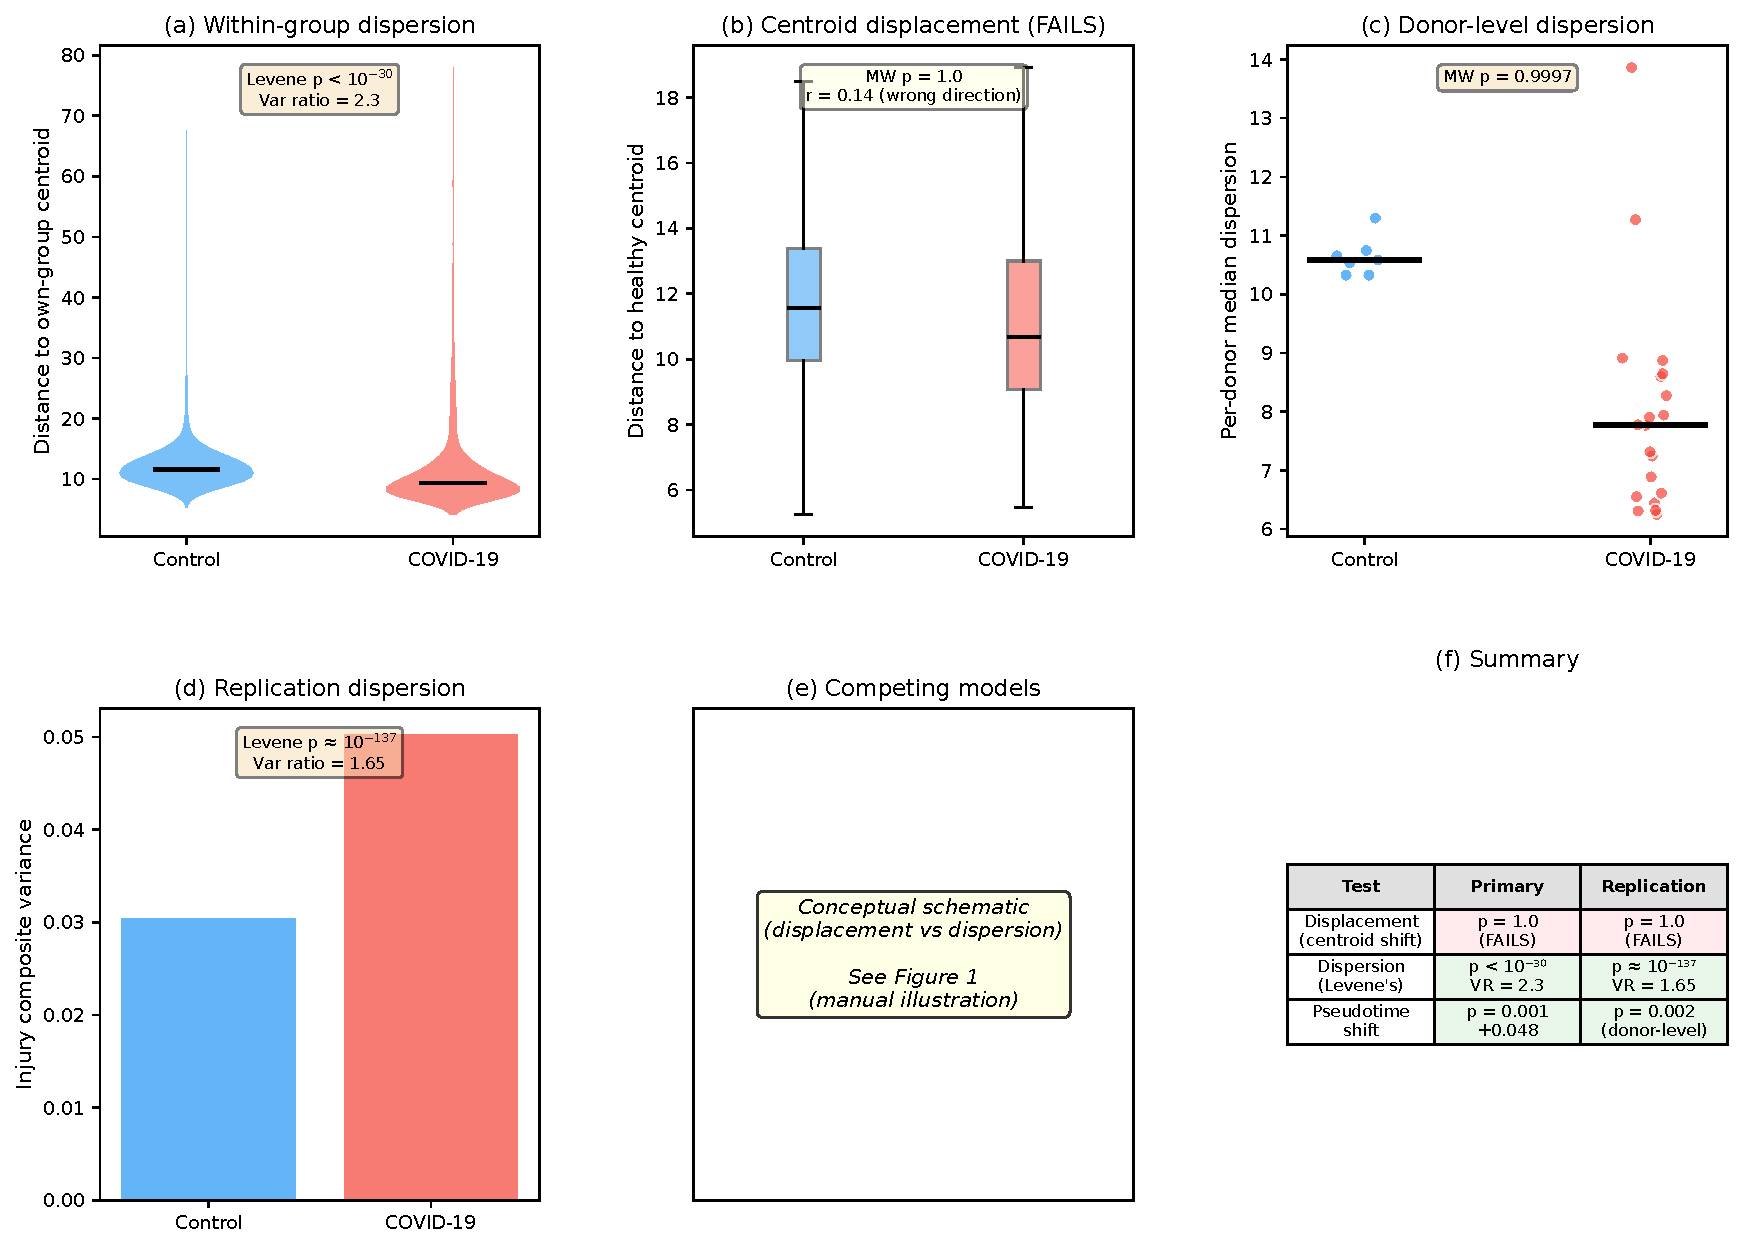
\includegraphics[width=\textwidth]{fig3_dispersion_centerpiece.pdf}
\caption{\textbf{Dispersion-dominated loss of state coherence.} (a) Within-group distance-to-centroid distributions (Levene $p < 10^{-30}$; ratio 2.3$\times$). (b) Displacement test ($p = 1.0$). (c) Donor-level within-donor dispersion. (d) Replication cohort. (e) Summary statistics.}
\end{figure}

\subsection{Result 3: Pseudotime Shift Supported}

COVID-19 cells are enriched at higher pseudotime positions along the injury trajectory.

\begin{center}
\small
\begin{tabular}{ll}
\toprule
Metric & Value \\
\midrule
Median pseudotime (COVID) & 0.111 \\
Median pseudotime (Healthy) & 0.063 \\
Observed difference & $+0.048$ ($\sim$5\% of $[0,1]$ range) \\
Permutation $p$-value & 0.001 (1,000 iterations) \\
Leave-one-donor-out & Direction preserved 27/27 \\
Post-Harmony shift & $+0.125$ (2.6$\times$ amplification) \\
Palantir cross-validation & $+0.028$ (same direction) \\
\bottomrule
\end{tabular}
\end{center}

Three robustness checks build confidence in this modest effect:
\begin{enumerate}
\item \textbf{Leave-one-donor-out}: Removing each of the 27 donors one at a time, the direction was preserved in all 27 iterations. No single donor drives the result.
\item \textbf{Harmony amplification}: After fixing the batch-correction bug, the shift increases 2.6-fold, indicating that uncorrected donor effects were attenuating the true signal.
\item \textbf{Cross-algorithm agreement}: Palantir, an independent trajectory algorithm, produces a shift of the same sign and comparable magnitude.
\end{enumerate}

\begin{figure}[H]
\centering
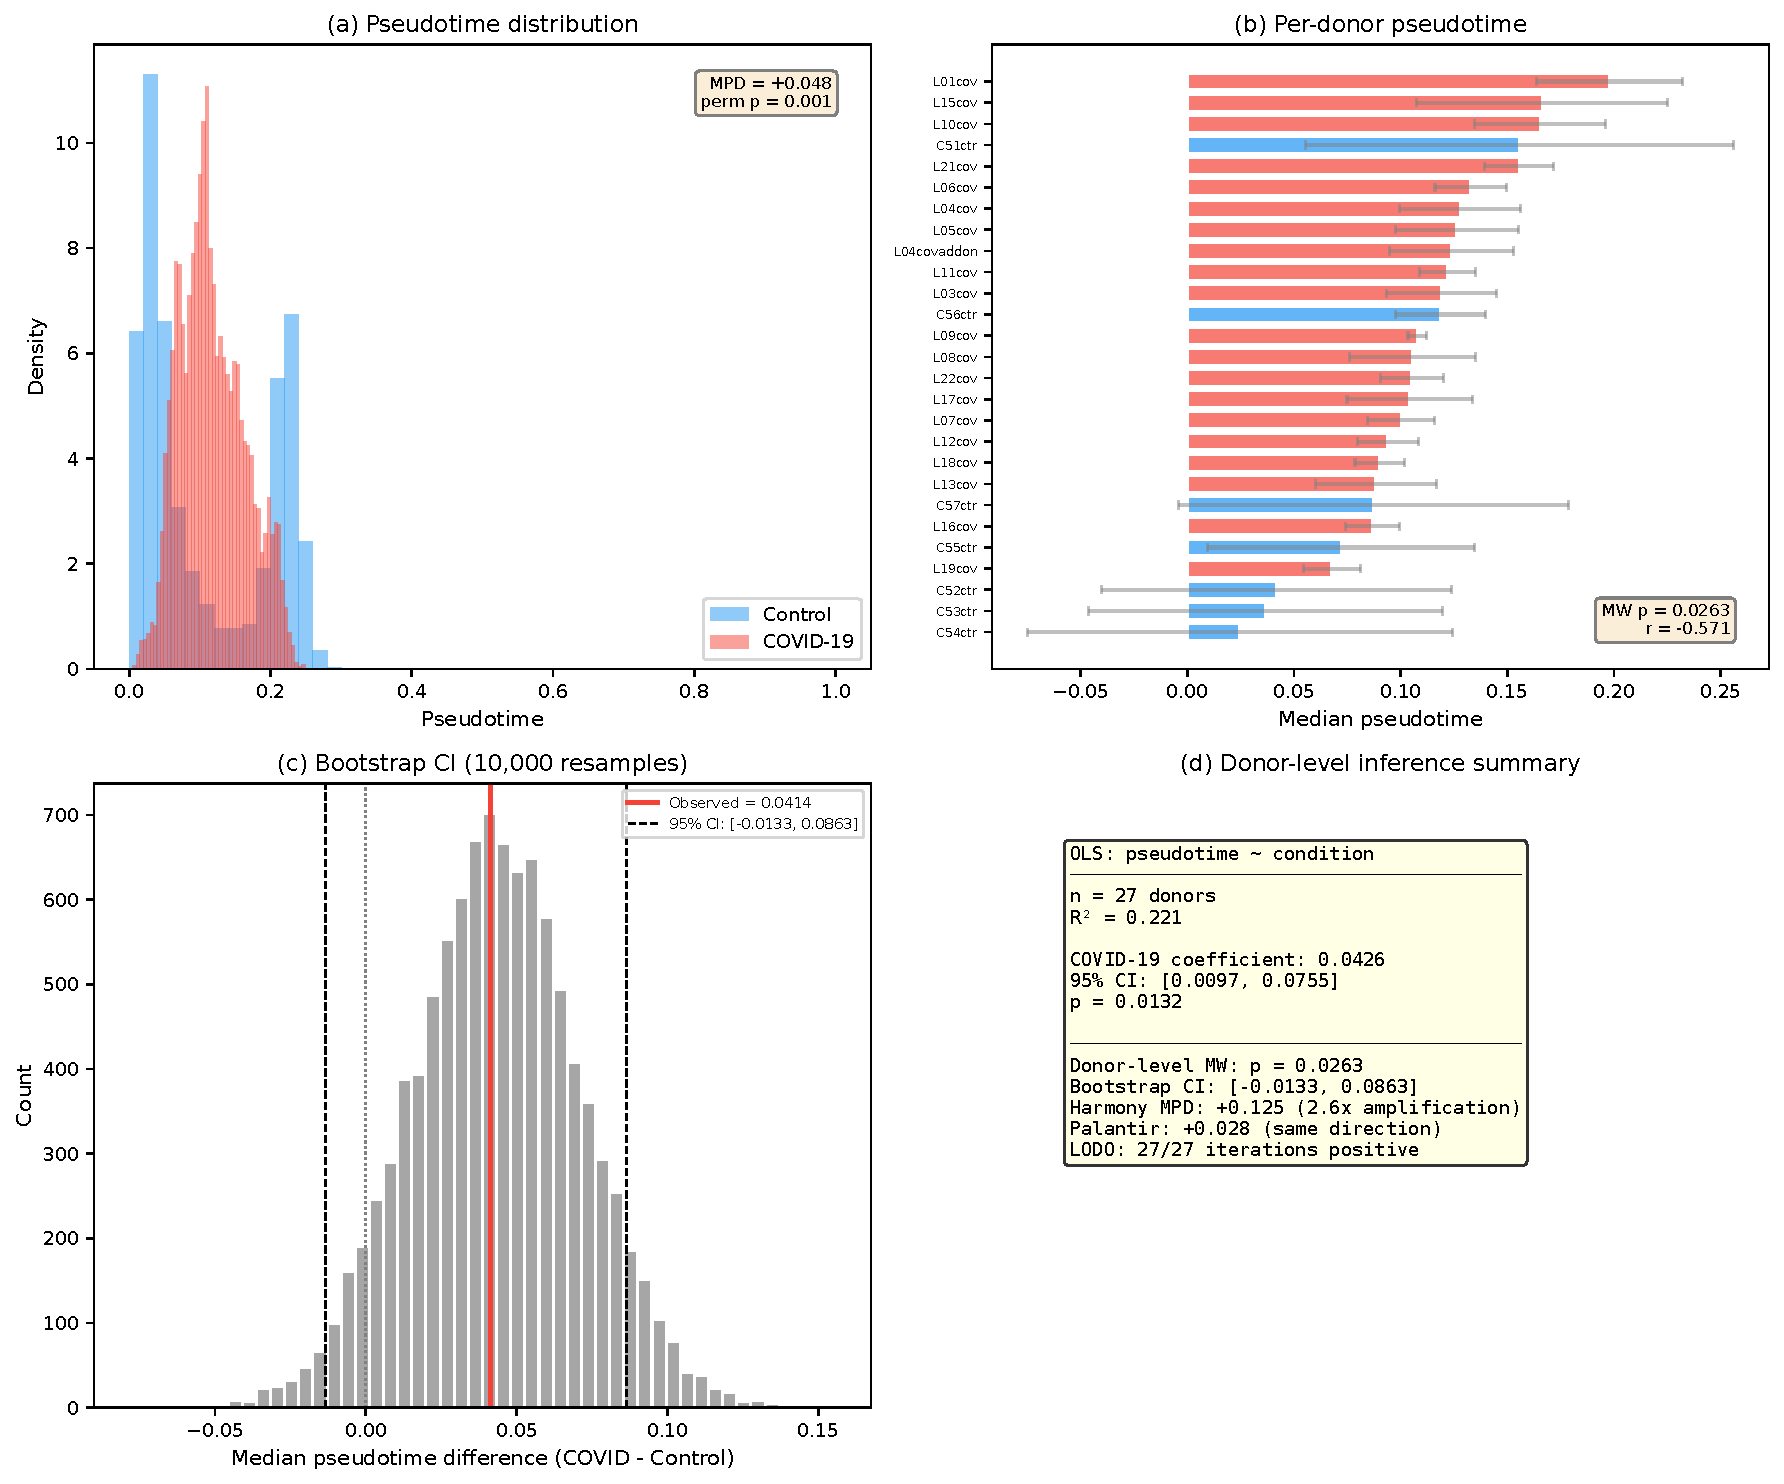
\includegraphics[width=\textwidth]{fig4_donor_pseudotime.pdf}
\caption{\textbf{Donor-level pseudotime analysis.} Per-donor median pseudotime, bootstrap CI, and OLS model.}
\end{figure}

\subsection{Result 4: Donor-Level Analysis --- A Surprising Twist}

Donor-level modeling reveals a nuanced picture that refines the main finding.

\paragraph{Donor-level OLS regression.}
\begin{center}
\small
\begin{tabular}{ll}
\toprule
Metric & Value \\
\midrule
COVID coefficient ($\beta$) & $+0.043$ \\
95\% CI & $[0.010, 0.076]$ \\
$p$-value & 0.013 \\
$R^2$ & 0.22 \\
$n$ (donors) & 27 \\
\bottomrule
\end{tabular}
\end{center}

Being a COVID-19 donor is associated with 0.043 units higher median pseudotime, and condition explains 22\% of donor-level variance.

\paragraph{The donor-level dispersion paradox.} At the cell level, COVID-19 cells are 2.3$\times$ more dispersed. But at the donor level, COVID-19 donors have \emph{lower} within-donor dispersion (median 7.77 vs 10.58 for healthy donors).

The resolution: individual COVID-19 donors are not internally messier. Each donor's cells form a relatively tight cluster, but each cluster sits in a \emph{different} region of injury space. One donor's cells may be dominated by senescence; another's by interferon response; another's by oxidative stress. Pooling all COVID-19 cells creates the appearance of high dispersion because the pool mixes cells from different injury regions.

This refines the biological interpretation: the heterogeneity is \textbf{between donors} (each patient responds differently to the virus), not \textbf{within donors} (individual patients having internally chaotic cells). The ``fan-out'' is a population-level phenomenon arising from patient-specific injury trajectories.

\subsection{Result 5: Portable State Scores}

Marker-threshold approaches for identifying transitional cells (e.g., KRT8$^+$/CLDN4$^+$) fail to transfer across cohorts due to differences in normalization, sequencing depth, and annotation. We developed six continuous state scores:

\begin{center}
\small
\begin{tabular}{llr}
\toprule
Score & Definition & AUC (transitional) \\
\midrule
AT2 identity & Mean of 9 AT2 markers & 0.323 \\
AT1 identity & Mean of 8 AT1 markers & 0.375 \\
Transitional & Mean of transitional markers & 0.441 \\
Injury composite & Mean of 6 injury programs & 0.630 \\
\textbf{Coherence loss} & Distance from healthy centroid & \textbf{0.972} \\
Repair failure & Transitional $-$ 0.5(AT2 + AT1) & 0.730 \\
\bottomrule
\end{tabular}
\end{center}

The coherence-loss score---simply the Euclidean distance from each cell to the centroid of healthy cells in PCA space---achieves near-perfect discrimination (AUC = 0.972) for annotated transitional cells. It requires no marker thresholds, just a distance calculation.

All six scores separate COVID-19 from healthy with $p < 10^{-300}$ in the replication cohort. Geometry-based scores transfer where marker thresholds fail.

\subsection{Result 6: Mechanistic Decomposition --- What Drives the Fan-Out?}

Linear regression of distance-to-healthy-centroid on the eight program scores ($R^2 = 0.115$) identified the biological programs responsible for the dispersion:

\begin{center}
\small
\begin{tabular}{lr}
\toprule
Program & Coefficient \\
\midrule
Senescence & $+6.83$ (largest contributor) \\
Oxidative stress & $+3.83$ \\
NF-$\kappa$B inflammatory & $+1.95$ \\
AT2 identity & $-1.13$ \\
AT1 identity & $-1.02$ \\
\bottomrule
\end{tabular}
\end{center}

The fan-out is driven by divergent activation of stress and senescence programs. Cells that retain their homeostatic identity (negative coefficients) stay near the healthy centroid. Cells that activate senescence, oxidative stress, or NF-$\kappa$B scatter furthest from healthy.

A repair-stall analysis showed that in healthy cells, the ratio of differentiation to apoptosis scores remains favorable at late pseudotime---cells complete the AT2-to-AT1 transition. In COVID-19 cells, apoptosis overtakes differentiation at late pseudotime, consistent with cells that initiate repair but are diverted toward death before reaching the AT1 endpoint.

\subsection{Result 7: Transitional Cells --- Enriched but Not Portable}

The ECM-high transitional population was 3.1-fold enriched in COVID-19 in the primary atlas (8.5\% vs 2.7\%; $\chi^2$ $p < 10^{-30}$). These cells sit at intermediate pseudotime positions and express KRT8 and CLDN4, consistent with damage-associated transient progenitors.

However, this enrichment does \textbf{not} replicate cross-cohort. Applying the same KRT8$^+$/CLDN4$^+$ threshold in the replication cohort gives the opposite result: COVID-19 had \emph{fewer} cells above the threshold (22.9\% vs 47.6\% in controls; 0.48$\times$ enrichment). This failure demonstrates that marker-threshold cell-state definitions are not portable across studies with different protocols and normalization.

\begin{figure}[H]
\centering
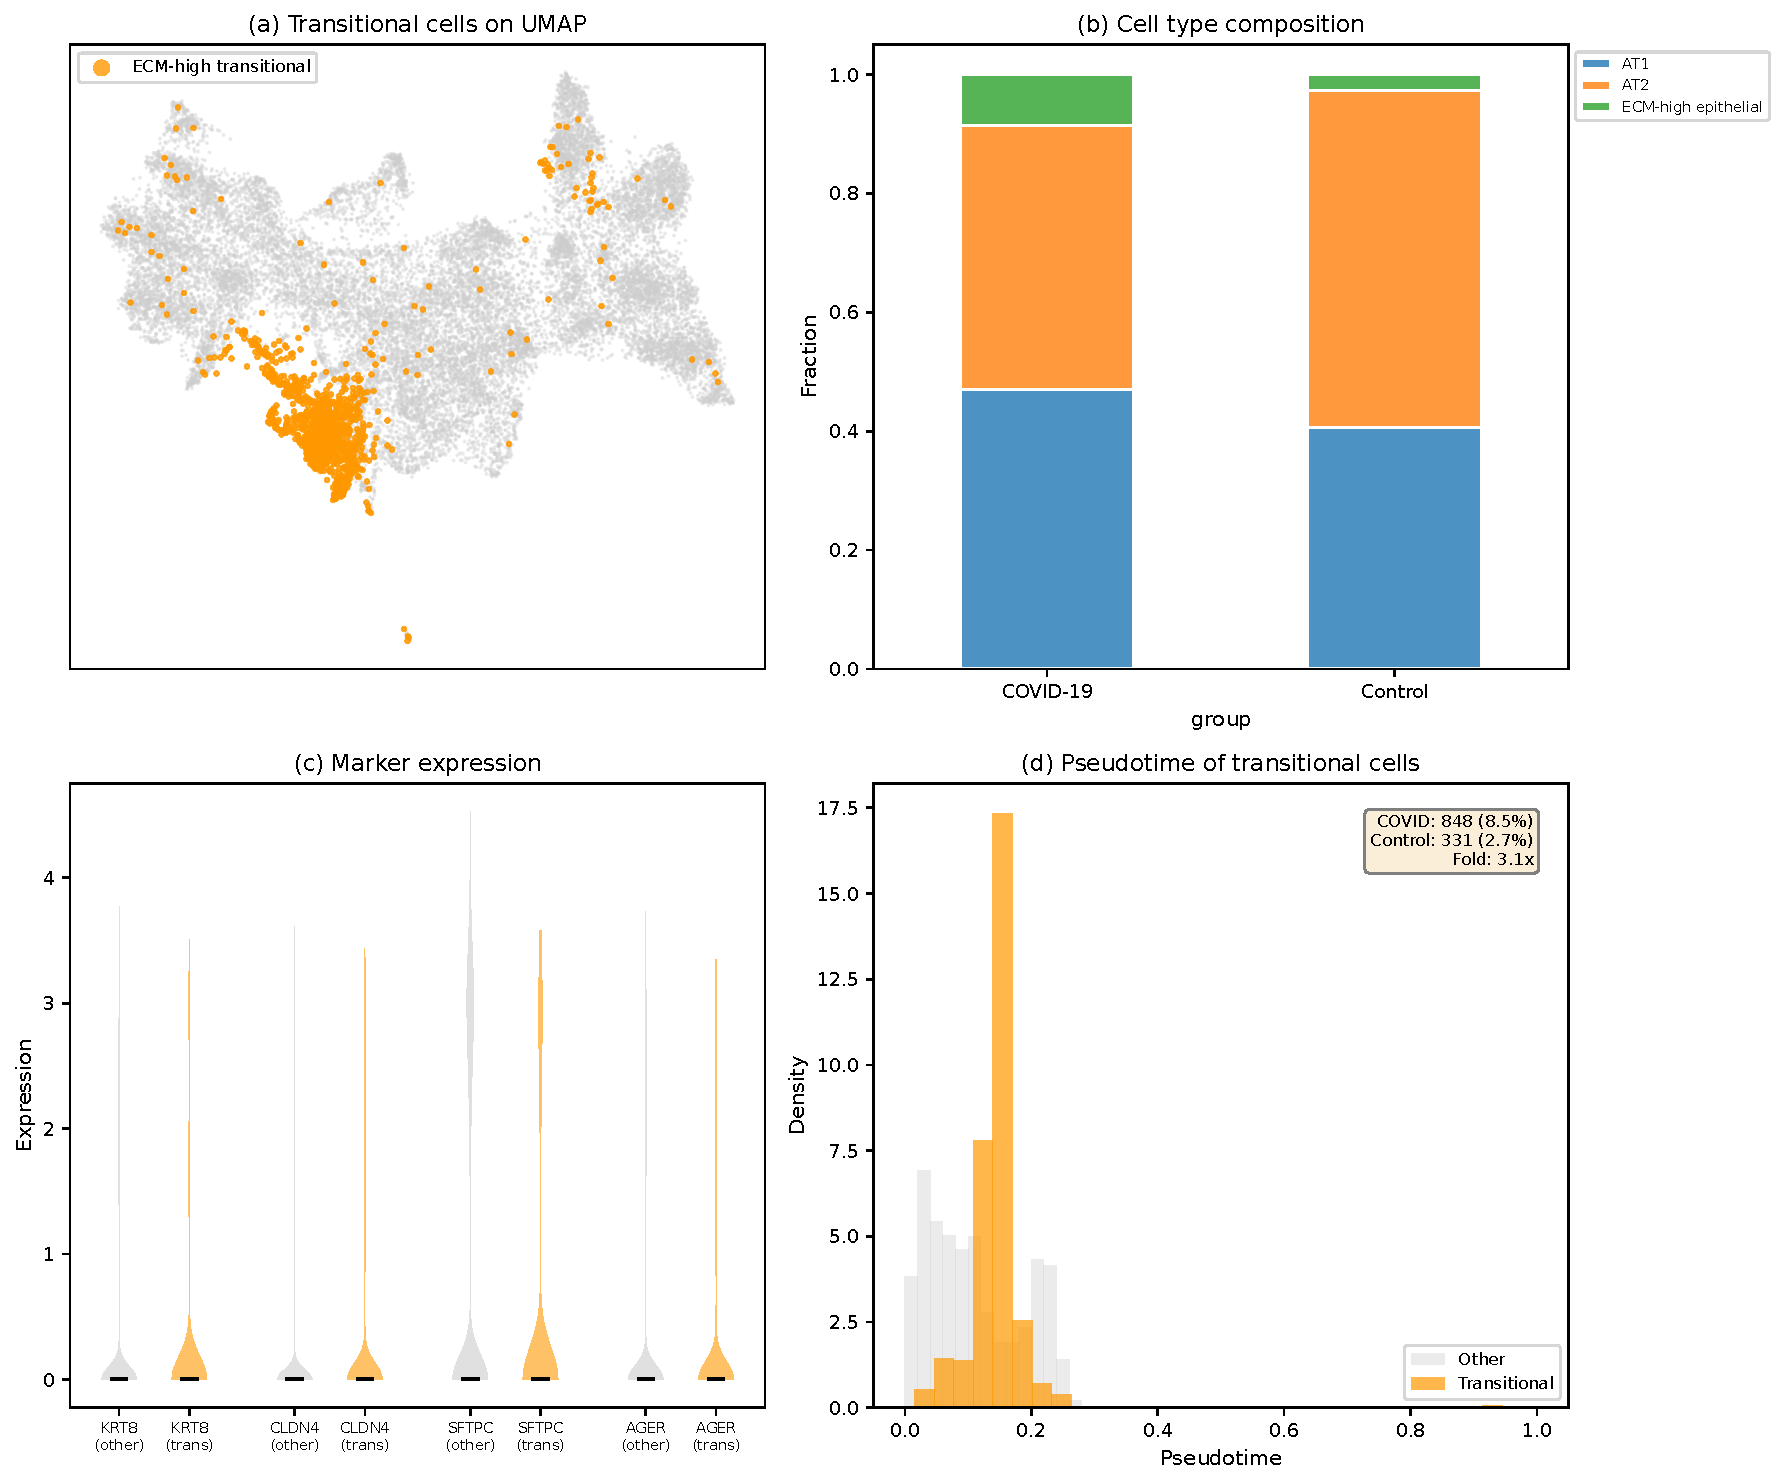
\includegraphics[width=\textwidth]{fig5_transitional.pdf}
\caption{\textbf{Transitional cell compartment.} (a) UMAP highlighting transitional cells. (b) Composition by condition. (c) Marker expression. (d) Pseudotime density by cell type.}
\end{figure}


% ============================================================================
\section{Robustness Testing: Ten Ablations}
% ============================================================================

An ablation changes one pipeline choice and checks whether the conclusion survives. We performed ten:

\begin{center}
\small
\begin{longtable}{p{3cm}p{8cm}p{3cm}}
\toprule
Ablation & What was changed & Outcome \\
\midrule
\endfirsthead
\toprule
Ablation & What was changed & Outcome \\
\midrule
\endhead
1. AT2-only & Dropped AT1 and transitional cells & Sign flip on displacement \\
2. Alternative embeddings & UMAP/diffmap variants & Shift \& dispersion persist \\
3. Harmony vs uncorrected & Post-bug-fix batch correction & 2.6$\times$ amplification \\
4. Drop apoptosis genes & Removed apoptosis from manifold & Signal not driven by apoptosis \\
5. Alternative roots & 4 different pseudotime roots & Stable for 3 of 4 \\
6. Broader epithelial & Added airway cells & Shift abolished (alveolar-specific) \\
7. Leave-one-donor-out & Removed 1 donor at a time ($\times$27) & Direction preserved 27/27 \\
8. Alternative programs & Swapped gene lists & Fine ordering inverts \\
9. Palantir & Different trajectory algorithm & Direction preserved (+0.028) \\
10. Permutation & Shuffled labels $\times$1,000 & $p = 0.001$ \\
\bottomrule
\end{longtable}
\end{center}

\begin{figure}[H]
\centering
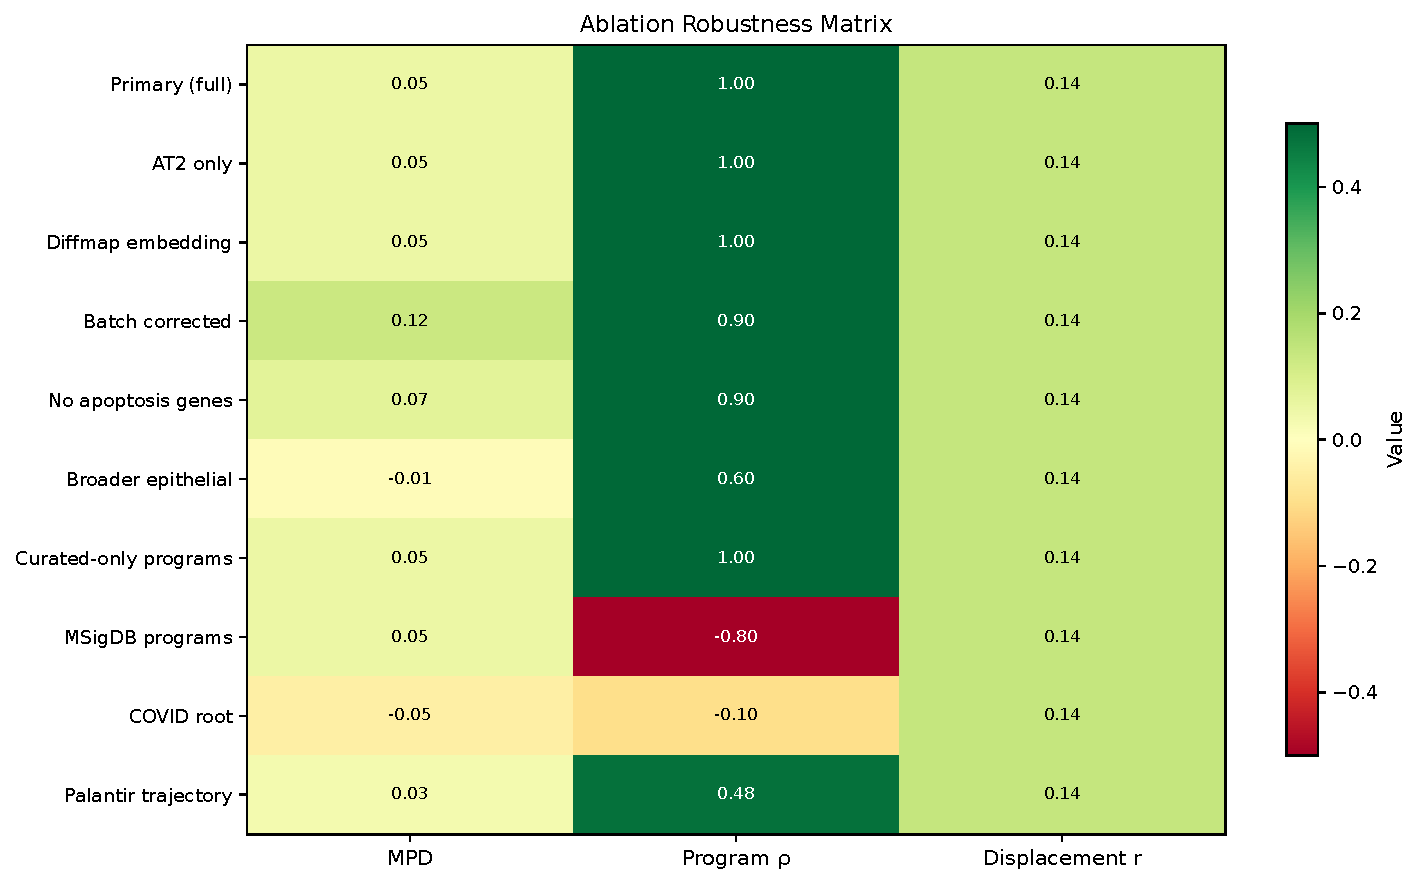
\includegraphics[width=0.9\textwidth]{fig6_ablation_matrix.pdf}
\caption{\textbf{Ablation robustness matrix.} Dispersion and pseudotime direction: robust across all ablations. Fine program ordering: fragile.}
\end{figure}

\paragraph{Summary of robustness.}
\begin{itemize}
\item \textbf{Robust}: Dispersion (survives all 10 ablations), pseudotime direction (survives all alveolar-compartment ablations), displacement failure (never becomes significant)
\item \textbf{Fragile}: Fine-grained program ordering (inverts under different gene lists), trajectory specificity (abolished when airway cells included)
\end{itemize}


% ============================================================================
\section{Independent Replication}
% ============================================================================

The replication cohort provides the definitive test of portability. Results are summarized in the following table:

\begin{center}
\small
\begin{tabular}{llll}
\toprule
Finding & Primary Atlas & Replication (618 donors) & Verdict \\
\midrule
Dispersion (Levene) & $p < 10^{-30}$, ratio 2.3$\times$ & $p \approx 10^{-137}$, ratio 1.65$\times$ & \textbf{Replicates strongly} \\
Pseudotime direction & perm.\ $p = 0.001$ & donor-level $p = 0.002$ & \textbf{Replicates} \\
Centroid displacement & fails ($p = 1.0$) & fails ($p = 1.0$) & \textbf{Failure replicates} \\
KRT8$^+$/CLDN4$^+$ DATP & 3.1$\times$ enriched & 0.48$\times$ (reversed) & \textbf{Does NOT replicate} \\
State scores (all 6) & all significant & all $p < 10^{-300}$ & \textbf{Replicate strongly} \\
\bottomrule
\end{tabular}
\end{center}

The pattern is clear: \textbf{geometric findings} (dispersion, donor-level trajectory direction) are portable across cohorts and methods. \textbf{Annotation-dependent findings} (marker thresholds, fine program ordering) are atlas-specific.


% ============================================================================
\section{Summary of Evidence}
% ============================================================================

\begin{center}
\small
\begin{tabular}{lcccc}
\toprule
Finding & Primary & Ablations & Replication & Verdict \\
\midrule
Dispersion & $p < 10^{-30}$ & 10/10 robust & $p \approx 10^{-137}$ & \textbf{Strong} \\
Pseudotime shift & $p = 0.001$ & 27/27 LOO & donor $p = 0.002$ & \textbf{Robust} \\
Donor-level OLS & $p = 0.013$ & --- & --- & \textbf{Supported} \\
Centroid displacement & $p = 1.0$ & 10/10 fails & $p = 1.0$ & \textbf{Ruled out} \\
DATP threshold & 3.1$\times$ & --- & reversed & \textbf{Not portable} \\
Fine program order & varies & inverts & --- & \textbf{Fragile} \\
\bottomrule
\end{tabular}
\end{center}

Not everything worked, and we report this honestly. Knowing what does not work is as scientifically valuable as knowing what does.


% ============================================================================
\section{Conclusions}
% ============================================================================

\subsection{The Main Conclusion}

Lethal COVID-19 does not push alveolar epithelial cells coherently away from the healthy state. Instead, it \textbf{fans them outward} across heterogeneous injury states---driven by divergent senescence, oxidative stress, and inflammatory programs---while each donor's cells occupy a different region of injury space. The strongest, most portable finding is \textbf{within-group dispersion}, which replicates across 35 datasets and 618 donors.

\subsection{The Refined Biological Story}

The cell-level dispersion arises from between-donor heterogeneity: each COVID-19 patient's cells respond to the virus in a relatively coordinated way, but different patients occupy different regions of injury space. One patient may be dominated by senescence, another by interferon response, another by oxidative stress. When cells from all patients are pooled, the aggregate looks highly dispersed---but within any single patient, cells are internally coherent. The ``loss of state coherence'' is a population-level phenomenon, not a per-patient phenomenon.

Among cells that initiate the AT2-to-AT1 repair trajectory, COVID-19 cells are more likely to be diverted toward apoptosis rather than completing the differentiation to AT1. The repair system starts but fails to finish.

\subsection{Key Methodological Takeaways}

Six lessons that generalize beyond this specific project:

\begin{enumerate}
\item \textbf{Pre-register opposing hypotheses.} Design tests where one outcome rules out a specific mechanism. A failing test is informative, not negative.
\item \textbf{Test dispersion, not just displacement.} For heterogeneous disease states, within-group variance captures what centroid displacement misses.
\item \textbf{Use donor-level pseudobulk.} The sample size is the number of donors, not cells. Cells from one donor are not independent.
\item \textbf{Use continuous state scores, not marker thresholds.} Thresholds break across cohorts; geometry-based distances don't.
\item \textbf{Run ablations.} They catch bugs (the Harmony orientation fix is exhibit A) and distinguish robust from fragile findings.
\item \textbf{Report honestly what fails.} Showing that DATP marker enrichment doesn't replicate is as valuable as showing that dispersion does.
\end{enumerate}


% ============================================================================
\section{Limitations}
% ============================================================================

\begin{enumerate}
\item \textbf{Post-mortem, lethal cases only.} No mild or moderate COVID-19 cases are available. The findings describe the worst-case endpoint.
\item \textbf{Small donor sample size.} 27 donors (7 vs 20) is small. The donor-level bootstrap 95\% CI for pseudotime difference marginally includes zero ($[-0.013, +0.086]$). The 618-donor replication addresses this partially.
\item \textbf{Pseudotime is an ordering, not a clock.} No claims about elapsed hours or disease stages.
\item \textbf{Narrow replication panel.} 84 genes is sufficient for scoring programs and computing dispersion but too narrow for independent manifold reconstruction.
\item \textbf{Fine program ordering is fragile.} Swapping gene lists inverts the ordering. This is hypothesis-generating only.
\item \textbf{DATP marker thresholds don't transfer.} Retracted as a cross-cohort finding.
\item \textbf{Post-mortem confounding.} Peri-mortem hypoxia, ischemia, and medication effects may influence stress and apoptosis program scores. Some of the signal may reflect dying in general, not COVID-19 specifically.
\item \textbf{No non-COVID ARDS controls.} Comparing COVID-19 against healthy donors (not against other causes of death) limits specificity claims.
\end{enumerate}


% ============================================================================
\section{Software and Reproducibility}
% ============================================================================

\begin{center}
\small
\begin{tabular}{ll}
\toprule
Component & Version \\
\midrule
Python & 3.12.3 \\
Scanpy & 1.12.1 \\
AnnData & 0.12.10 \\
NumPy & 2.4.3 \\
SciPy & 1.17.1 \\
pandas & 2.3.3 \\
harmonypy & 0.2.0 \\
palantir & 1.4.4 \\
Random seed & 42 \\
\bottomrule
\end{tabular}
\end{center}

All code is organized in \texttt{src/} with orchestration in \texttt{scripts/}. Every parameter is in \texttt{config.yaml}. The full pipeline can be reproduced with:

\begin{verbatim}
python scripts/run_pipeline.py --step all       # Primary pipeline
python scripts/run_v3_analyses.py               # Donor models, scores, mechanisms
bash scripts/ablations/rerun_all.sh             # All ten ablations
python scripts/replication/fetch_replication.py  # Fetch replication data
python scripts/replication/analyze_replication.py # Replication analysis
python scripts/generate_v3_figures.py           # Generate all figures
\end{verbatim}


% ============================================================================
\section{References}
% ============================================================================

\begin{thebibliography}{99}
\small

\bibitem{Adams2020}
Adams, T.~S., et al. (2020). Single-cell RNA-seq reveals ectopic and aberrant lung-resident cell populations in idiopathic pulmonary fibrosis. \textit{Science Advances}, 6(28):eaba1983.

\bibitem{Barkauskas2013}
Barkauskas, C.~E., et al. (2013). Type 2 alveolar cells are stem cells in adult lung. \textit{J.\ Clin.\ Invest.}, 123(7):3025--3036.

\bibitem{Borczuk2020}
Borczuk, A.~C., et al. (2020). COVID-19 pulmonary pathology. \textit{Modern Pathology}, 33(11):2156--2168.

\bibitem{Delorey2021}
Delorey, T.~M., et al. (2021). COVID-19 tissue atlases reveal SARS-CoV-2 pathology and cellular targets. \textit{Nature}, 595(7865):107--113.

\bibitem{Habermann2020}
Habermann, A.~C., et al. (2020). Single-cell RNA sequencing reveals profibrotic roles of distinct epithelial and mesenchymal lineages. \textit{Science Advances}, 6(28):eaba1972.

\bibitem{Haghverdi2016}
Haghverdi, L., et al. (2016). Diffusion pseudotime robustly reconstructs lineage branching. \textit{Nature Methods}, 13(10):845--848.

\bibitem{Hou2020}
Hou, Y.~J., et al. (2020). SARS-CoV-2 reverse genetics reveals a variable infection gradient. \textit{Cell}, 182(2):429--446.e14.

\bibitem{Kobayashi2020}
Kobayashi, Y., et al. (2020). Persistence of a regeneration-associated, transitional alveolar epithelial cell state. \textit{Nature Cell Biology}, 22(8):934--946.

\bibitem{Korsunsky2019}
Korsunsky, I., et al. (2019). Fast, sensitive and accurate integration of single-cell data with Harmony. \textit{Nature Methods}, 16(12):1289--1296.

\bibitem{Melms2021}
Melms, J.~C., et al. (2021). A molecular single-cell lung atlas of lethal COVID-19. \textit{Nature}, 595(7865):114--119.

\bibitem{Setty2019}
Setty, M., et al. (2019). Characterization of cell fate probabilities in single-cell data with Palantir. \textit{Nature Biotechnology}, 37(4):451--460.

\bibitem{Strunz2020}
Strunz, M., et al. (2020). Alveolar regeneration through a Krt8$^+$ transitional stem cell state. \textit{Nature Communications}, 11(1):3559.

\bibitem{Wendisch2021}
Wendisch, D., et al. (2021). SARS-CoV-2 infection triggers profibrotic macrophage responses. \textit{Cell}, 184(26):6243--6261.e27.

\bibitem{Wolf2018}
Wolf, F.~A., Angerer, P., Theis, F.~J. (2018). SCANPY: large-scale single-cell gene expression data analysis. \textit{Genome Biology}, 19(1):15.

\bibitem{Ziegler2020}
Ziegler, C.~G.~K., et al. (2020). SARS-CoV-2 receptor ACE2 is an interferon-stimulated gene. \textit{Cell}, 181(5):1016--1035.e19.

\end{thebibliography}

\end{document}
